\begin{frame}[plain,noframenumbering]
    \centering
    \scalebox{5}{PART II}
\end{frame}

\begin{frame}[plain,noframenumbering]
    \centering
    \scalebox{3}{Dangling References}
\end{frame}

\section{Dangling References}

\begin{frame}[fragile]{Will it compile?}
    \inputcpplisting{snippet22a}

\end{frame}

\begin{frame}[fragile]{Will it invoke undefined behavior?}
    \inputcpplisting{snippet22b}

    \hfill \ldots binding a reference to a temporary???
\end{frame}

\begin{frame}[fragile]{Temporary object lifetime extension}
    \inputcpplisting{snippet22b}

    \href{https://en.cppreference.com/w/cpp/language/lifetime}{\texttt{cppreference.com}: \enquote{The lifetime of a temporary object may be extended by binding to a const lvalue reference or to an rvalue reference (since C++11).}}
\end{frame}

\begin{frame}[fragile]{Q: What is the output of the program?}
    \inputcpplisting{snippet29}
\end{frame}

\begin{frame}[fragile]{A: \texttt{a1b1a2xb2}}
    \begin{columns}
        \begin{column}{.55\textwidth}
            \inputcpplisting{snippet29}
        \end{column}
        \begin{column}{.4\textwidth}
            \textbf{Dangling reference!!!}
            \begin{itemize}
                \item lifetime extension only for result of the temporary expression, \textbf{not any sub-expression}
                \item use \href{https://clang.llvm.org/docs/AddressSanitizer.html}{address sanitizer}!    
            \end{itemize}
        \end{column}
    \end{columns}
\end{frame}

\begin{frame}[plain,noframenumbering]
    \centering
    \scalebox{2.}{contrived?}
\end{frame}

\begin{frame}[fragile]{Reference lifetime extension}
    \begin{center}
        \scalebox{.7}{(derived from \href{https://abseil.io/tips/107}{\texttt{abseil.io}: Tip of the Week \#107: \enquote{Reference Lifetime Extension})}}
    \end{center}

    \begin{lstlisting}
std::vector<std::string_view> explode(const std::string& s);

for (std::string_view s: explode(str_cat("oo", "ps"))) { // WRONG!
    [...]
    \end{lstlisting}
\end{frame}

\begin{frame}[fragile]{Q: What is the output of the program?}
    \begin{columns}
        \begin{column}{.45\textwidth}
            \inputcpplisting{snippet30}
        \end{column}
        \begin{column}{.5\textwidth}
            \only<2>{%
            \textbf{Dangling reference!!!}
            \begin{itemize}
                \item \texttt{std::vector} needs to reallocate all the space the second time an element is pushed 
                \item use \href{https://clang.llvm.org/docs/AddressSanitizer.html}{address sanitizer}!    
            \end{itemize}}
        \end{column}
    \end{columns}
\end{frame}

\begin{frame}[plain,noframenumbering]
    \centering
    \scalebox{3}{\texttt{std::move} in the wild}
\end{frame}

\section{\texttt{std::move} in the wild}

\begin{frame}[fragile]{Moving \texttt{std::string}}
    \centering
    \scalebox{.7}{(derived from \href{https://youtu.be/oTMSgI1XjF8}{CppCon 2019: \textit{Ben Deane} \enquote{Everyday Efficiency: In-Place Construction (Back to Basics?)})}}

    \begin{lstlisting}
static void cp_small_str(benchmark::State& state) {
    for (auto _ : state) {
        std::string original("small");
        benchmark::DoNotOptimize(original);
        std::string copied = original;
        benchmark::DoNotOptimize(copied);
    }
}
BENCHMARK(cp_small_str);
    \end{lstlisting}

    \begin{lstlisting}
static void mv_small_str(benchmark::State& state) {
    for (auto _ : state) {
        std::string original("small");
        benchmark::DoNotOptimize(original);
        std::string moved = std::move(original);
        benchmark::DoNotOptimize(moved);
    }
}
BENCHMARK(mv_small_str);
    \end{lstlisting}
\end{frame}

\begin{frame}[fragile]{Moving \texttt{std::string}}
    \centering
    \scalebox{.7}{(derived from \href{https://youtu.be/oTMSgI1XjF8}{CppCon 2019: \textit{Ben Deane} \enquote{Everyday Efficiency: In-Place Construction (Back to Basics?)})}}

    \begin{lstlisting}
static void cp_long_str(benchmark::State& state) {
    for (auto _ : state) {
        std::string original("this is too long for short string optimization");
        benchmark::DoNotOptimize(original);
        std::string copied = original;
        benchmark::DoNotOptimize(copied);
    }
}
BENCHMARK(cp_long_str);
    \end{lstlisting}

    \begin{lstlisting}
static void mv_long_str(benchmark::State& state) {
    for (auto _ : state) {
        std::string original("this is too long for short string optimization");
        benchmark::DoNotOptimize(original);
        std::string moved = std::move(original);
        benchmark::DoNotOptimize(moved);
    }
}
BENCHMARK(mv_long_str);
    \end{lstlisting}
\end{frame}

\begin{frame}{Moving \texttt{std::string}}
    \centering
    \scalebox{1.5}{Quick Bench result}

    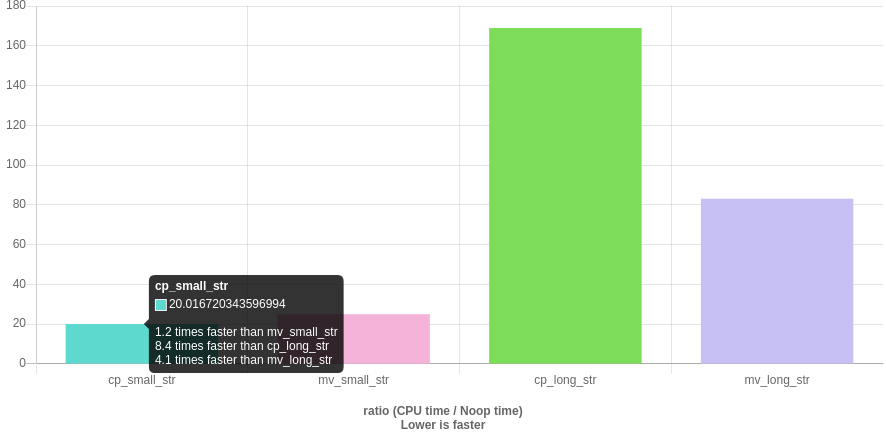
\includegraphics[width=.9\textwidth]{benchmark_str_cp_mv.png}

    Quick Bench: \href{http://quick-bench.com/l_4Ith4ZvZbSE0UIfIQXVpkg84A}{\texttt{tinyurl.com/yybmdngv}}
\end{frame}

\begin{frame}[fragile]{Moving \texttt{std::string}}
    \centering

    \begin{columns}[t]
        \begin{column}{.45\textwidth}
            \begin{block}{Copy small \texttt{std::string}}
                \begin{enumerate}
                    \item copy stack allocated data
                \end{enumerate}
            \end{block}
        \end{column}
        \begin{column}{.45\textwidth}
            \begin{block}{Move small \texttt{std::string}}
                \begin{enumerate}
                    \item copy stack allocated data
                    \item set string length of moved string to zero
                \end{enumerate}
            \end{block}
        \end{column}
    \end{columns}

    \vspace{5mm}

    \begin{center}
        \scalebox{1.5}{$\hookrightarrow$ moving is not necessarily better than copying!}
    \end{center}
\end{frame}

\begin{frame}[fragile]{Moving \texttt{std::map}}
    \textbf{Did they forget to mark the move ctor \texttt{noexcept}?} \only<2>{\textcolor{vertexDarkRed}{No!}}

    \begin{columns}[t]
        \begin{column}{.45\textwidth}
            \begin{lstlisting}[numbers=none]
// since C++11
std:map(const std:map&&)

// until C++17
std:map& operator(std:map&&)

// since C++17
std:map& operator(std:map&&) noexcept
            \end{lstlisting}
        \end{column}
        \begin{column}{.5\textwidth}
            \begin{itemize}
                \item<2> Move ctor needs to allocate new sentinel node, because moved from container must still be a valid container (albeit in an unspecified state)
                \item<2> Move assignment can swap, thus no need to allocate
            \end{itemize}
        \end{column}
    \end{columns}

    \only<2>{%
    \begin{center}
        \scalebox{1.5}{$\hookrightarrow$ move ctor of \texttt{std::map} allocates heap space!}

        \scalebox{.8}{(Billy O'Neal: \href{https://twitter.com/MalwareMinigun/status/1165310509022736384}{\texttt{twitter.com/MalwareMinigun/status/1165310509022736384})}}
    \end{center}}
\end{frame}

\begin{frame}[fragile]{Moving \texttt{std::map}}
    \begin{lstlisting}
static void rvo(benchmark::State& state) {
    for (auto _ : state) {
        auto m = []() -> std::map<int, int> {
            std::map<int, int> m{{0, 42}};
            return m;
        }();
        benchmark::DoNotOptimize(m);
    }
}
BENCHMARK(rvo);
    \end{lstlisting}

    \begin{lstlisting}
static void fmove(benchmark::State& state) {
    for (auto _ : state) {
        auto m = []() -> std::map<int, int> {
            std::map<int, int> m{{0, 42}};
            return std::move(m);
        }();
        benchmark::DoNotOptimize(m);
    }
}
BENCHMARK(fmove);
    \end{lstlisting}
\end{frame}
\begin{frame}[fragile]{Moving \texttt{std::map}}
    \begin{lstlisting}
static void copy(benchmark::State& state) {
    for (auto _ : state) {
        std::map<int, int> m{{0, 42}};
        benchmark::DoNotOptimize(m);
        auto m2 = m;
        benchmark::DoNotOptimize(m2);
    }
}
BENCHMARK(copy);
    \end{lstlisting}
\end{frame}

\begin{frame}{Moving \texttt{std::map}}
    \centering
    \scalebox{1.5}{Quick Bench result}

    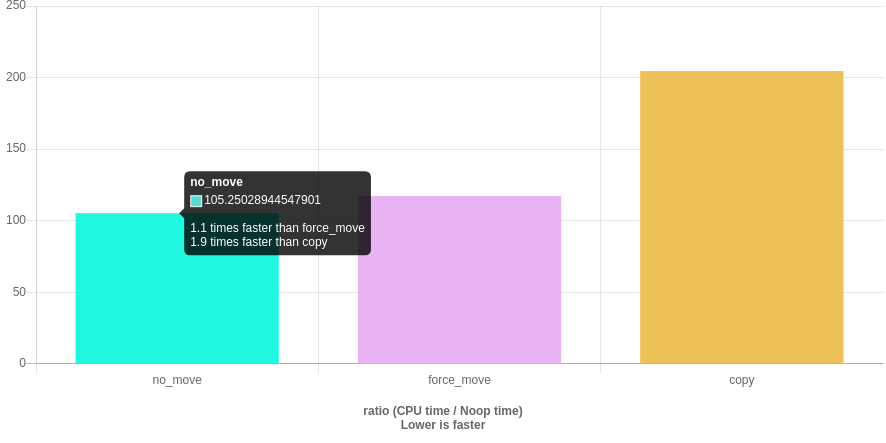
\includegraphics[width=.9\textwidth]{benchmark_map_mv.png}

    Quick Bench: \href{http://quick-bench.com/7L-__vxvraDDacztJoalrjBrMUA}{\texttt{tinyurl.com/y57egvjp}}
\end{frame}

\begin{frame}[plain,noframenumbering]
    \centering
    \scalebox{5}{Why?}
\end{frame}

\begin{frame}[fragile]{Does this code bother anyone?}
    \inputcpplisting{snippet3}
\end{frame}

\begin{frame}[plain,noframenumbering]
    \centering
    \scalebox{2}{Interlude}

    \scalebox{3}{What happens on \texttt{return}?}
\end{frame}

\section{What Happens on \texttt{return}?}

\begin{frame}[fragile]{Will it compile?}
    \inputcpplisting{snippet8}
\end{frame}


\begin{frame}[fragile]{Implicit conversion to the function return type}
    \begin{columns}
        \begin{column}{.55\textwidth}
            \textbf{Implicit conversion}
            \begin{itemize}
                \item \ldots if ctor is \textbf{not} marked \texttt{explicit}
                \item Examples: 
                \begin{itemize}
                    \item \href{https://en.cppreference.com/w/cpp/utility/optional/optional}{\texttt{std::optional(T\&\&)}}
                    \item \href{https://en.cppreference.com/w/cpp/string/basic_string/basic_string}{\texttt{std::string(const char*)}}
                \end{itemize}
            \end{itemize}
        \end{column}
        \begin{column}{.35\textwidth}
            \inputcpplisting{snippet27}
        \end{column}
    \end{columns}
\end{frame}

\begin{frame}[fragile]{Q: What is the output of the program?}
    \begin{center}
        Compiler flags: \texttt{-std=c++14 -fno-elide-constructors}
    \end{center}

    \inputcpplisting{snippet4a}
\end{frame}


\begin{frame}[fragile]{Q: What is the output of the program?}
    \begin{center}
        Compiler flags: \texttt{-std=c++17}
    \end{center}

    \inputcpplisting{snippet4b}
\end{frame}


\begin{frame}[plain,noframenumbering]
    \centering
    \scalebox{5}{\only<1>{Why?}
    }

    \only<2>{Ben Deane: \enquote{Perhaps the most important optimization the compiler does}}
\end{frame}

\begin{frame}{Copy Elision}
    \begin{columns}
        \begin{column}{.45\textwidth}
            \inputcpplisting{snippet10}
        \end{column}
        \begin{column}{.5\textwidth}
            Mandatory elision of copy/move operations since \texttt{C++17}):
            \begin{itemize}
                \item Return statement: when operand is a \texttt{prvalue} of same class type as return type
                \item Initialization of a variable: when initializer expression is a \texttt{prvalue} of same class type as the variable type
            \end{itemize}
        \end{column}
    \end{columns}
    \ldots even if the copy/move constructor and the destructor has observable side-effects!
    \vspace{.5cm}

    \centering
    \scalebox{1.5}{\textbf{Rule of thumb: avoid naming return values}}
\end{frame}

\section{RVO in Depth}

\begin{frame}[plain,noframenumbering]
    \centering
    \scalebox{3}{RVO in Depth}
\end{frame}

\begin{frame}[fragile]{\texttt{C++} Objects in Assembly}
    \begin{columns}[t]
        \begin{column}{.45\textwidth}
            \inputcpplisting{snippet20}
        \end{column}
        \begin{column}{.45\textwidth}
            \begin{lstlisting}[language={},morekeywords={rdi},numbers=none]
  | main:
14|   push rbp
14|   mov rbp, rsp
14|   sub rsp, 16
14|   mov dword ptr [rbp - 4], 0
15|   lea rdi, [rbp - 16]
15|   mov esi, 1
15|   mov edx, 2
15|   mov ecx, 3
15|   call S::S(int, int, int)
16|   lea rdi, [rbp - 16]
16|   call S::sum()
16|   mov dword ptr [rbp - 4], eax
17|   lea rdi, [rbp - 16]
17|   call S::~S()
17|   mov eax, dword ptr [rbp - 4]
17|   add rsp, 16
17|   pop rbp
17|   ret
            \end{lstlisting}
        \end{column}
    \end{columns}
\end{frame}

\begin{frame}[fragile]{\texttt{C++} Objects in Assembly}
    \begin{columns}[t]
        \begin{column}{.45\textwidth}
            \inputcpplisting{snippet20}
        \end{column}
        \begin{column}{.45\textwidth}
            \begin{lstlisting}[language={},morekeywords={rdi},numbers=none]
  | S::S(int, int, int):
 5|   push rbp
 5|   mov rbp, rsp
 5|   mov qword ptr [rbp - 8], rdi
 5|   mov dword ptr [rbp - 12], esi
 5|   mov dword ptr [rbp - 16], edx
 5|   mov dword ptr [rbp - 20], ecx
 5|   mov rax, qword ptr [rbp - 8]
 5|   mov ecx, dword ptr [rbp - 12]
 5|   mov dword ptr [rax], ecx
 5|   mov ecx, dword ptr [rbp - 16]
 5|   mov dword ptr [rax + 4], ecx
 5|   mov ecx, dword ptr [rbp - 20]
 5|   mov dword ptr [rax + 8], ecx
 5|   pop rbp
 5|   ret
            \end{lstlisting}
        \end{column}
    \end{columns}
\end{frame}

\begin{frame}[fragile]{\texttt{C++} Objects in Assembly}
    \begin{columns}[t]
        \begin{column}{.45\textwidth}
            \inputcpplisting{snippet20}
        \end{column}
        \begin{column}{.45\textwidth}
            \begin{lstlisting}[language={},morekeywords={rdi},numbers=none]
  | S::sum():
 9|   push rbp
 9|   mov rbp, rsp
 9|   mov qword ptr [rbp - 8], rdi
 9|   mov rax, qword ptr [rbp - 8]
10|   mov ecx, dword ptr [rax]
10|   add ecx, dword ptr [rax + 4]
10|   add ecx, dword ptr [rax + 8]
10|   mov eax, ecx
10|   pop rbp
10|   ret
            \end{lstlisting}
        \end{column}
    \end{columns}
\end{frame}

\begin{frame}[fragile]{RVO in Assembly}
    \begin{columns}[t]
        \begin{column}{.45\textwidth}
            \inputcpplisting{snippet7}
        \end{column}
        \begin{column}{.45\textwidth}
            \begin{lstlisting}[language={},morekeywords={rdi},numbers=none]
# g92 -fno-elide-constructors
  | g():
  |   [...]
14|   lea rax, [rbp-20]
14|   mov rdi, rax
14|   call f()
14|   lea rdx, [rbp-20]
14|   lea rax, [rbp-24]
14|   mov rsi, rdx
14|   mov rdi, rax
14|   call S::S(S&&)
14|   lea rax, [rbp-20]
14|   mov rdi, rax
14|   call S::~S()
15|   mov ebx, DWORD PTR [rbp-24]
14|   lea rax, [rbp-24]
14|   mov rdi, rax
14|   call S::~S()
15|   mov eax, ebx
  |   [...]      
            \end{lstlisting}
        \end{column}
    \end{columns}
\end{frame}

\begin{frame}[fragile]{RVO in Assembly}
    \begin{columns}[t]
        \begin{column}{.45\textwidth}
            \inputcpplisting{snippet7}
        \end{column}
        \begin{column}{.45\textwidth}
            \begin{lstlisting}[language={},morekeywords={rdi},numbers=none]
# g92 -fno-elide-constructors
  | f():
  |   [...]
 9|   mov QWORD PTR [rbp-24], rdi
10|   lea rax, [rbp-4]
10|   mov esi, 42
10|   mov rdi, rax
10|   call S::S(int)
10|   lea rdx, [rbp-4]
10|   mov rax, QWORD PTR [rbp-24]
10|   mov rsi, rdx
10|   mov rdi, rax
10|   call S::S(S&&)
10|   lea rax, [rbp-4]
10|   mov rdi, rax
10|   call S::~S()
  |   [...]      
            \end{lstlisting}
        \end{column}
    \end{columns}
\end{frame}

\begin{frame}[fragile]{RVO in Assembly}
    \begin{columns}[t]
        \begin{column}{.45\textwidth}
            \begin{lstlisting}[language={},morekeywords={rdi}]
# g92 -fno-elide-constructors
f():
  [...]
  mov QWORD PTR [rbp-24], rdi
  lea rax, [rbp-4]
  mov esi, 42
  mov rdi, rax
  call S::S(int)
  lea rdx, [rbp-4]
  mov rax, QWORD PTR [rbp-24]
  mov rsi, rdx
  mov rdi, rax
  call S::S(S&&)
  lea rax, [rbp-4]
  mov rdi, rax
  call S::~S()
  nop
  mov rax, QWORD PTR [rbp-24]
  leave
  ret
            \end{lstlisting}
        \end{column}
        \begin{column}{.45\textwidth}
            \begin{lstlisting}[language={},morekeywords={rdi}]
# g92
f():
  [...]
  mov QWORD PTR [rbp-8], rdi
  mov rax, QWORD PTR [rbp-8]
  mov esi, 42
  mov rdi, rax
  call S::S(int)
  mov rax, QWORD PTR [rbp-8]
  leave
  ret
            \end{lstlisting}
        \end{column}
    \end{columns}
\end{frame}

\begin{frame}[fragile]{RVO in Assembly}
    \begin{columns}[t]
        \begin{column}{.45\textwidth}
            \begin{lstlisting}[language={},morekeywords={rdi}]
# g92 -fno-elide-constructors
g():
  [...]
  lea rax, [rbp-20]
  mov rdi, rax
  call f()
  lea rdx, [rbp-20]
  lea rax, [rbp-24]
  mov rsi, rdx
  mov rdi, rax
  call S::S(S&&)
  lea rax, [rbp-20]
  mov rdi, rax
  call S::~S()
  mov ebx, DWORD PTR [rbp-24]
  lea rax, [rbp-24]
  mov rdi, rax
  call S::~S()
  mov eax, ebx
  [...]      
            \end{lstlisting}
        \end{column}
        \begin{column}{.45\textwidth}
            \begin{lstlisting}[language={},morekeywords={rdi}]
# g92
g():
  [...]
  lea rax, [rbp-20]
  mov rdi, rax
  call f()
  mov ebx, DWORD PTR [rbp-20]
  lea rax, [rbp-20]
  mov rdi, rax
  call S::~S()
  mov eax, ebx
            \end{lstlisting}
        \end{column}
    \end{columns}
\end{frame}

\begin{frame}[fragile]{(N)RVO or no (N)RVO?}
    \inputcpplisting{snippet21}
    \begin{itemize}
        \item \texttt{f1}: \only<1>{???}
        \item \texttt{f2}: \only<1>{???}
        \item \texttt{f3}: \only<1>{???}
        \item \texttt{f4}: \only<1>{???}
    \end{itemize}
\end{frame}

\begin{frame}[fragile]{(N)RVO or no (N)RVO?}
    \inputcpplisting{snippet25}
    \begin{itemize}
        \item \texttt{f1}: \only<1>{???}
        \item \texttt{f2}: \only<1>{???}
        \item \texttt{f3}: \only<1>{???}
    \end{itemize}
\end{frame}

\begin{frame}[fragile]{(N)RVO or no (N)RVO?}
    \inputcpplisting{snippet23}

\end{frame}

\begin{frame}[fragile]{(N)RVO or no (N)RVO?}
    \inputcpplisting{snippet26}
    \begin{itemize}
        \item \texttt{f1}: \only<1>{???}
        \item \texttt{f2}: \only<1>{???}
    \end{itemize}

\end{frame}

\begin{frame}[fragile]{(N)RVO or no (N)RVO?}
    \inputcpplisting{snippet24}
    \begin{itemize}
        \item \texttt{g1}: \only<1>{???}
        \item \texttt{g2}: \only<1>{???}
        \item \texttt{g3}: \only<1>{???}
        \item \texttt{g4}: \only<1>{???}
    \end{itemize}
\end{frame}

\begin{frame}[fragile]{(N)RVO or no (N)RVO?}
    \begin{center}
        \scalebox{.7}{(derived from \href{https://youtu.be/ZxWjii99yao}{CppCon 2019: \textit{Jason Turner} \enquote{Great C++ is\_trivial}})}
    \end{center}

    \textbf{No (N)RVO in any of these examples!}
    \begin{lstlisting}
S g1() { auto [s1, s2] = f(); return s1; } // copy
S g2() { auto&& [s1, s2] = f(); return s1; } // copy: no implicit move yet (?)
S g3() { auto [s1, s2] = f(); return std::move(s1); } // move
S g4() { auto&& [s1, s2] = f(); return std::move(s1); } // move
    \end{lstlisting}
    
    \hfill \ldots \texttt{return std::move} is not always bad

    \textbf{Why?} Structured bindings:
    \begin{itemize}
        \item Creation of temporary object \texttt{e}
        \item Like a reference: structured binding is an alias into \texttt{e}
    \end{itemize}
\end{frame}

\begin{frame}{Implicit move}
    \begin{center}
        \scalebox{1.5}{\texttt{return std::move} is not yet necessarily a code smell}

        (use \texttt{-Wpessimizing-move})
    \end{center}

    \href{https://en.cppreference.com/w/cpp/language/return}{\textbf{Automatic move from local variables and parameters \underline{if}:}}
    \begin{itemize}
        \item return expression names a variable whose type is either
        \begin{itemize}
            \item an object type or (since \texttt{C++11})
            \item an rvalue reference to object type (since \texttt{C++20}${}^{\textcolor{vertexDarkRed}\star}$)
        \end{itemize}
        \item \ldots and that variable is declared
        \begin{itemize}
            \item in the body or
            \item as a parameter of
        \end{itemize}
        \item \ldots the innermost enclosing function or lambda expression
    \end{itemize}

    ${}^{\textcolor{vertexDarkRed}\star}$ \scalebox{.8}{\href{http://www.open-std.org/jtc1/sc22/wg21/docs/papers/2019/p1825r0.html}{\texttt{P1825R0}} (not yet implemented in GCC or Clang: \href{https://en.cppreference.com/w/cpp/compiler_support}{cppreference.com/w/cpp/compiler\_support})}
\end{frame}

\begin{frame}[plain,noframenumbering]
    \centering
    \scalebox{3}{Perfect Backwarding}
\end{frame}

\section{Perfect Backwarding}

\begin{frame}[fragile]{Forwarding Values and Preserving Value Category}
    \centering

    \scalebox{.7}{(derived from \href{https://youtu.be/hwT8K3-NH1w}{CppCon 2018: \textit{Hayun Ezra Chung} \enquote{Forwarding Values... and Backwarding Them Too?})}}

    \only<1>{\inputcpplisting{snippet11a}}%
    \only<2>{\inputcpplisting{snippet11b}}%
    \only<3>{\inputcpplisting{snippet11c}}%
\end{frame}

\begin{frame}[fragile]{Backwarding Values and Preserving Value Category}
    \only<1>{\inputcpplisting{snippet18a}}%
    \only<2>{\inputcpplisting{snippet18b}}%
\end{frame}

\begin{frame}[fragile]{Backwarding Values and Preserving Value Category}
    \textbf{Q:} Why is this a bad idea?
    \begin{lstlisting}
auto&& visit(auto visitor) {
    auto&& result = visitor(resource);
    return result;
}
    \end{lstlisting}
    
    \only<2>{%
    \textbf{A:} Dangling reference for

    \centering
    \texttt{visit([](Resource\& r) -> Resource \{ return r; \}));}

    \vspace{.5cm}

    \begin{center}
        \scalebox{1.5}{\texttt{auto\&\&} is always a reference!}
    \end{center}}
\end{frame}

\begin{frame}[fragile]{Backwarding Values and Preserving Value Category}
    \only<1>{\inputcpplisting{snippet12a}}%
    \only<2>{\inputcpplisting{snippet12b}}
\end{frame}

\begin{frame}[fragile]{Backwarding Values and Preserving Value Category}
    \only<1>{\inputcpplisting{snippet13a}}%
    \only<2>{\inputcpplisting{snippet13b}}
\end{frame}

\begin{frame}[fragile]{Backwarding Values and Preserving Value Category}
    \centering
    \only<1>{\inputcpplisting{snippet14a}}%
    \only<2,3>{%
        \only<3>{\textbf{\textcolor{vertexDarkRed}{error:}} cannot bind rvalue reference of type \enquote{Resource\&\&} to lvalue of type \enquote{Resource}}%
        \inputcpplisting{snippet14b}%
    }%
    \only<4>{\inputcpplisting{snippet14c}}
\end{frame}

\begin{frame}[fragile]{Backwarding Values and Preserving Value Categroy}
    \centering
    \scalebox{1.5}{How do we fuse these implementations?}

    \begin{lstlisting}
Resource visit(auto visitor) {
    Resource result = visitor(resource);
    return result;
}

Resource& visit(auto visitor) {
    Resource& result = visitor(resource);
    return result;
}

Resource&& visit(auto visitor) {
    Resource&& result = visitor(resource);
    return static_cast<Resource&&>(result);
}
    \end{lstlisting}

    \begin{lstlisting}
Target(rm.visit([](Resource& r) -> Resource { return r; }));
Target(rm.visit([](Resource& r) -> Resource& { return r; }));
Target(rm.visit([](Resource& r) -> Resource&& { return std::move(r); }));
    \end{lstlisting}
\end{frame}

\begin{frame}[fragile]{Backwarding Values and Preserving Value Categroy}
    \centering
    \scalebox{1.5}{How do we fuse these implementations?}

    \begin{lstlisting}
Resource visit(auto visitor) {
    Resource result = visitor(resource);
    return result;
}

Resource& visit(auto visitor) {
    Resource& result = visitor(resource);
    return result;
}

Resource&& visit(auto visitor) {
    Resource&& result = visitor(resource);
    return static_cast<Resource&&>(result);
}
    \end{lstlisting}

    \begin{lstlisting}
decltype(auto) visit(auto visitor) {
    decltype(auto) result = visitor(resource);
    return static_cast<decltype(result)>(result);
}
    \end{lstlisting}
\end{frame}

\begin{frame}[fragile,plain,noframenumbering]
    \centering
    \scalebox{.7}{(derived from \href{https://youtu.be/hwT8K3-NH1w}{CppCon 2018: \textit{Hayun Ezra Chung} \enquote{Forwarding Values... and Backwarding Them Too?})}}

    \inputcpplisting{snippet15}
\end{frame}

\begin{frame}[plain,noframenumbering]
    \centering
    \scalebox{5.}{\color{vertexDarkRed}$*$}
\end{frame}

\begin{frame}[fragile]{Q: What is the output of the program?}
    \inputcpplisting{snippet16a}
\end{frame}


\begin{frame}[fragile]{Q: What is the output of the program?}
    \inputcpplisting{snippet16b}
\end{frame}


\begin{frame}[fragile]{Missing (N)RVO}
    \begin{lstlisting}
struct Resource {
    [...]
    Resource(const Resource&) { std::cout << 'a'; }
};

Resource visit(auto visitor) {
    Resource result = visitor(resource);
    return static_cast<Resource>(result);
}
    \end{lstlisting}

    \textbf{Neither RVO nor NRVO!}
    \begin{itemize}
        \item \texttt{static\_cast} is not the name of a variable (c-style cast does not work either)
        \item compiler cannot elide observable side effects of copy construction
        \item \enquote{Solution}
        \begin{itemize}
            \item remove explicit cast, or
            \item remove side effect (\texttt{std::cout})
        \end{itemize}
    \end{itemize}
\end{frame}

\begin{frame}[fragile]{Missing (N)RVO}
    \begin{lstlisting}
template <typename T>
decltype(auto) visit(T visitor) {
    decltype(auto) result = visitor(resource);
    if constexpr (std::is_same_v<decltype(result), Resource&&>) {
        return std::move(result);
    } else {
        return result;
    }
}
    \end{lstlisting}

    \hfill \ldots works for GCC (without \texttt{auto} concept), not for Clang though
\end{frame}

\begin{frame}[fragile]{Missing (N)RVO}
    \begin{lstlisting}
template <typename T>
static constexpr bool returns_rref = std::is_same_v<std::invoke_result_t<T, Resource&>, Resource&&>;

template <typename T, std::enable_if_t<returns_rref<T>, int> = 0>
decltype(auto) visit(T visitor) {
    decltype(auto) result = visitor(resource);
    return std::move(result);
}

template <typename T, std::enable_if_t<not returns_rref<T>, int> = 0>
decltype(auto) visit(T visitor) {
    decltype(auto) result = visitor(resource);
    return result;
}
    \end{lstlisting}

    \hfill \ldots still, no NRVO with Clang but this time due to the deduced return type!
\end{frame}

\begin{frame}[fragile]{Missing (N)RVO}
    \begin{lstlisting}
template <typename T>
static constexpr bool returns_rref = std::is_same_v<std::invoke_result_t<T, Resource&>, Resource&&>;

template <typename T, std::enable_if_t<returns_rref<T>, int> = 0>
decltype(auto) visit(T visitor) {
    decltype(auto) result = visitor(resource);
    return std::move(result);
}

template <typename T, std::enable_if_t<not returns_rref<T>, int> = 0>
auto visit(T visitor) -> decltype(visitor(resource)) {
    decltype(auto) result = visitor(resource);
    return result;
}
    \end{lstlisting}

    \hfill \ldots now works for GCC and Clang!
\end{frame}

\begin{frame}[fragile,plain,noframenumbering]
    \inputcpplisting{snippet17}
\end{frame}

\begin{frame}[fragile,plain,noframenumbering]
    \scalebox{3.}{More things that don't work}
\end{frame}

\begin{frame}[fragile]{Missing (N)RVO}
    \inputcpplisting{snippet19a}

    \hfill \ldots works with GCC, fails with Clang
\end{frame}


\begin{frame}[fragile]{Missing (N)RVO}
    \inputcpplisting{snippet19b}

    \hfill \ldots works with Clang, fails with GCC
\end{frame}

\begin{frame}[fragile]{Missing (N)RVO}
    \inputcpplisting{snippet19c}

    \hfill \ldots fails with GCC and Clang
\end{frame}

\begin{frame}{Conclusion}
    \begin{center}
        \scalebox{.7}{(shamelessly copied from \href{https://youtu.be/hwT8K3-NH1w}{CppCon 2018: \textit{Hayun Ezra Chung} \enquote{Forwarding Values... and Backwarding Them Too?})}}
    \end{center}
    
    \textbf{Forwarding}
    \begin{itemize}
        \item Parameter Type: \texttt{T\&\&}
        \item Function Argument: \texttt{std::forward<E>(e)}
        \item Alternatively: \texttt{static\_cast<decltype(e)\&\&>(e)}
    \end{itemize}

    \textbf{Backwarding}
    \begin{itemize}
        \item Parameter Type: \texttt{decltype(auto)}
        \item Function Argument: \texttt{decltype(e)(e)}
        \item Alternatively: \texttt{static\_cast<decltype(e)>(e)}$^*$
    \end{itemize}
\end{frame}
